% section | subsection | subsubsection | paragraph | subparagraph | verbatim | enumerate | item

% Just let it be an Article bro
\documentclass{article}

% Cover Metadata
\title{Developing The Opportunity}
\date{10 Oktober 2025}
\author{Maulana Hafidz Ismail}

% Image Setup
\usepackage{graphicx}
\usepackage{float}

% Link Setup
\usepackage{hyperref}
\usepackage{bookmark}

% Highlighting Setup
\usepackage{soul}
\usepackage{xcolor}
\sethlcolor{red!30}
\newcommand{\hlblue}[1]{\sethlcolor{cyan!30}\hl{#1}\sethlcolor{yellow}}

% Line Width
\sloppy
\setlength{\emergencystretch}{3em}
\hbadness=99999

% Code Syntax Setup
\usepackage{listings}
\usepackage{xcolor} % untuk warna
\lstset{
basicstyle=\ttfamily\small,
frame=single,
breaklines=true,
backgroundcolor=\color{gray!10},
keywordstyle=\color{blue},
commentstyle=\color{gray},
stringstyle=\color{red},
tabsize=2,
captionpos=b
}

% Start of the Article
\begin{document}

% Cover Page
\pagenumbering{gobble}
\maketitle
\newpage

% Table of Content Page
\tableofcontents
\newpage
\pagenumbering{arabic}

% Main Content
\section{Introduction to Entrepreneurship}
\subsection{Kewirausahaan di Perusahaan Besar}
Terdapat perdebatan tentang apakah perusahaan yang sudah mapan dapat bersikap kewirausahaan. Beberapa argumen menyatakan bahwa manajer di perusahaan besar perlu mengadopsi praktik kewirausahaan untuk tetap kompetitif.

\subsection{Inovasi Inkremental vs. Diskontinu}
Inovasi inkremental adalah perbaikan kecil pada produk yang sudah ada, sedangkan inovasi diskontinu adalah perubahan besar yang menciptakan produk baru. Contoh: iPhone asli sebagai inovasi diskontinu, sedangkan iPhone 6s sebagai inovasi inkremental.

\subsection{Ekplorasi vs. Eksploitasi}
Perusahaan sering terjebak dalam eksploitasi  (perbaikan kecil untuk pelanggan yang ada) dan perlu melakukan eksplorasi (mencari peluang baru) untuk bertahan dalam jangka panjang.

\subsection{Inovasi Disruptif}
Konsep ini menjelaskan bagaimana perusahaan baru dapat mengganggu pasar yang sudah ada dengan teknologi yang awalnya tidak memenuhi kebutuhan pelanggan, tetapi kemudian berkembang untuk memenuhi kebutuhan tersebut.

\subsection{Strategi untuk Mendorong Inovasi}
\begin{itemize}
    \item Pengembangan Internal: Memberikan waktu khusus untuk eksplorasi, seperti yang dilakukan oleh 3M dan Google.
    \item Kemitraan Strategis: Bekerja sama dengan perusahaan lain untuk berbagi teknologi dan pasar, seperti kemitraan Tesla dengan Toyota.
    \item Akuisisi: Mengakuisisi perusahaan lain untuk mendapatkan akses penuh ke teknologi dan sumber daya.
\end{itemize}

\subsection{Model Venture Creation}
model sederhana dari penciptaan usaha yang melibatkan beberapa aktor penting, seperti \textbf{entrepreneur} (pengusaha), \textbf{venture capital} (modal ventura), dan \textbf{perusahaan yang sudah} mapan.

\subsection{Peran Pengusaha}
Pengusaha adalah entitas yang mendirikan usaha dengan ide-ide baru. Mereka memerlukan pendanaan dari modal ventura untuk mengembangkan usaha yang memiliki potensi pertumbuhan tinggi.

\subsection{Aliran Modal dan Sumber Daya}
Terdapat aliran uang (dari modal ventura) dan aliran orang (profesional dari perusahaan mapan yang ingin mengejar inovasi) ke dalam konteks startup.

\subsection{Statistik Kewirausahaan}
Menurut Kauffman Foundation, hanya 0.3\% orang dewasa di AS yang menjadi pengusaha, tetapi mereka menciptakan banyak lapangan kerja, terutama di sektor usaha kecil.

\subsection{Unicorn}
Istilah "unicorn" merujuk pada startup yang memiliki valuasi lebih dari \$1 miliar. Meskipun jumlahnya masih sedikit, jumlah unicorn terus meningkat.

\subsection{Sektor Teknologi}
Sebagian besar nilai yang diciptakan dalam konteks startup berasal dari sektor teknologi, diikuti oleh sektor Kesehatan.

\subsection{Tipe-tipe Perusahaan}
\begin{itemize}
    \item Lifestyle Startups:

          Dijalankan sebagai hobi atau sumber pendapatan tambahan. Tujuannya bukan untuk skala besar, tetapi untuk menikmati kegiatan sambil menghasilkan uang.

    \item Small Businesses:

          Bisnis yang bertujuan untuk keberlanjutan dan tidak berfokus pada pertumbuhan cepat. Contoh: restoran, laundry, atau usaha kecil lainnya. Pendanaan biasanya berasal dari pinjaman atau investasi pribadi.

    \item High Growth Startups:

          Fokus pada pertumbuhan cepat dan skalabilitas. Memerlukan modal ventura atau investasi malaikat. Tujuannya bisa berupa IPO atau akuisisi oleh perusahaan besar.

    \item Intrapreneurship:

          Membangun inovasi dalam perusahaan yang sudah ada. Menggunakan sumber daya internal dan memiliki risiko yang lebih rendah.

    \item Social Ventures:

          Tujuan utama adalah menciptakan dampak sosial positif. Pendanaan berasal dari hibah, sumbangan, atau relawan.
\end{itemize}

\subsection{Peluang Kewirausahaan}
Perubahan teknologi dapat menciptakan peluang kewirausahaan, seperti munculnya Google dan Facebook berkat internet, atau Genentech berkat kemajuan DNA rekombinan. Namun, pengakuan terhadap peluang ini tidak menjamin kesuksesan komersial.

\subsection{Keputusan Penting}
Keberhasilan perusahaan tidak hanya bergantung pada pengenalan peluang, tetapi juga pada desain model bisnis, pemilihan sumber daya, dan kemampuan merekrut personel kunci.

\subsection{Ko-lokasi Geografis}
Banyak perusahaan teknologi terletak di daerah tertentu (misalnya, Silicon Valley) karena adanya konsentrasi pengetahuan dan investasi. Ini membantu dalam pengembangan perusahaan yang ingin memanfaatkan inovasi.

\subsection{Kekuatan Pasar dan Negosiasi}
Ukuran keuntungan yang dapat diperoleh dari inovasi dipengaruhi oleh kekuatan tawar dan kekuatan pasar. Hal ini dipengaruhi oleh kemampuan untuk mengontrol pengetahuan yang diciptakan, aset pelengkap, dan tahap evolusi industri.

\subsection{Desain Dominan}
Desain dominan, seperti iPhone, mempengaruhi bagaimana produk baru harus dirancang untuk bersaing di pasar. Pada awal evolusi industri, kontrol ide lebih penting, tetapi seiring waktu, kekuatan aset pelengkap menjadi lebih krusial.

\subsection{Definisi Impact Entrepreneurship}
Merupakan penciptaan perusahaan yang etis dan transparan, dengan fokus pada keuntungan dan dampak sosial serta lingkungan. Ini berbeda dari organisasi nirlaba karena tetap berorientasi pada profit.

\subsection{Triple Bottom Line}
Terdiri dari tiga aspek:
\begin{itemize}
    \item Profit: Keuntungan finansial.
    \item Social Impact: Dampak positif terhadap masyarakat.
    \item Environmental Impact: Dampak positif terhadap lingkungan.
\end{itemize}

\subsection{Contoh Impact Entrepreneurs}
\begin{itemize}
    \item Muhammad Yunus: Pendiri Grameen Bank yang menyediakan pinjaman kecil untuk masyarakat miskin di Bangladesh.
    \item Iqbal Quadir: Pendiri GrameenPhone yang memberikan akses telekomunikasi untuk meningkatkan pendapatan masyarakat.
\end{itemize}

\subsection{Tantangan dalam Scaling}
\begin{itemize}
    \item Kesulitan dalam memperluas jangkauan karena masalah biaya dan kompleksitas sosial.
    \item Pentingnya kemitraan dan pengaruh kebijakan untuk mengatasi hambatan.
\end{itemize}

\subsection{Pendanaan}
Impact entrepreneurs sering mencari sumber pendanaan yang lebih sabar, seperti yayasan filantropi dan dana ventura yang berfokus pada dampak sosial.

\subsection{Model Bisnis Tradisional vs. Sosial}
Perusahaan tradisional juga dapat mengadopsi misi sosial, seperti Warby Parker dan Toms, yang menerapkan model "beli satu, sumbang satu".

\subsection{Peran Venture Creation}
Venture creation dianggap sebagai kebaikan sosial karena menyediakan modal untuk menciptakan industri dan bisnis baru, yang pada gilirannya menciptakan lapangan kerja.

\subsection{Peluang Kewirausahaan}
Peluang sering kali ditemukan ketika seorang wirausahawan mengenali titik infleksi dalam teknologi, bukan dengan mencari masalah di pasar terlebih dahulu.

\subsection{Proses Pengujian Ide}
Penting untuk menguji ide dan melakukan pivot pada pasar, bukan pada produk, untuk menemukan pasar yang tepat untuk produk yang ditawarkan.

\subsection{Kualitas wirausahawan}
Wirausahawan yang sukses memiliki kemampuan untuk mengenali titik infleksi teknologi lebih awal dan fleksibilitas untuk mencoba berbagai pasar.

\subsection{Jaringan Pribadi}
Jaringan sangat penting dalam mendapatkan pendanaan dan bakat, tetapi tanpa traction di pasar, reputasi saja tidak cukup untuk menjamin kesuksesan.

\subsection{Kesalahan Umum}
Banyak tim membuat kesalahan dalam perekrutan sebelum mencapai product-market fit, karena sulit untuk menarik talenta terbaik pada tahap awal.

\subsection{Tantangan Perusahaan Besar}
Perusahaan besar sering kali menghadapi tantangan struktural seperti skala, hierarki, dan budaya yang dapat menghambat inovasi. Namun, perusahaan yang berkomitmen untuk inovasi dapat mengatasi tantangan ini.

\subsection{Karakteristik Karyawan}
Tidak semua orang memiliki jiwa kewirausahaan. Karyawan dengan kemampuan dan karakteristik yang beragam diperlukan untuk kesuksesan organisasi. Beberapa posisi memerlukan semangat kewirausahaan, sementara yang lain lebih cocok untuk stabilitas dan konsistensi.

\subsection{Pentingnya Kolaborasi}
Dalam lingkungan startup, kolaborasi dan toleransi terhadap risiko sangat penting. Karyawan harus mampu beradaptasi dengan perubahan dan berkontribusi dalam tim.

\subsection{Pendekatan Terhadap Inovasi}
Perusahaan dapat memilih untuk mengembangkan inovasi secara internal atau melalui akuisisi. Keberhasilan sering kali terjadi ketika perusahaan mengakuisisi bisnis yang sejalan dengan inti bisnis mereka.

\subsection{Mentoring dan Jaringan}
Memiliki mentor yang baik dan membangun jaringan yang kuat sangat penting untuk pengembangan karir dan kewirausahaan. Jaringan dapat memberikan akses ke pengetahuan, sumber daya, dan peluang.

\subsection{Kreativitas dan Inovasi}
Inovasi harus menjadi bagian dari budaya perusahaan. Karyawan didorong untuk berbagi ide dan berkontribusi pada proyek inovatif, dan perusahaan harus merayakan keberhasilan inovasi.

\newpage

\section{Opportunity Analysis}
\subsection{Kewirausahaan dan Ketidakpastian}
\begin{itemize}
    \item Kewirausahaan melibatkan mengambil risiko dan menghadapi ketidakpastian.
    \item Anda tidak bisa tahu dengan pasti apakah ide bisnis Anda akan berhasil.
\end{itemize}

\subsection{Tiga Kategori Ketidakpastian}
\begin{itemize}
    \item Fakta yang Diketahui: Informasi yang sudah pasti.
    \item Ketidakpastian: Situasi yang Anda tahu ada, tetapi hasilnya tidak pasti.
    \item Risiko yang Tidak Diketahui: Hal-hal yang bisa terjadi tanpa peringatan.
\end{itemize}

\subsection{Perencanaan untuk Mengurangi Ketidakpastian}
\begin{itemize}
    \item Rencanakan untuk mengubah ketidakpastian menjadi informasi yang lebih jelas.
    \item Perencanaan membantu Anda mengidentifikasi risiko dan mempersiapkan diri.
\end{itemize}

\subsection{Pembelajaran dan Adaptasi}
\begin{itemize}
    \item Startups perlu belajar dan beradaptasi seiring waktu.
    \item Perusahaan yang mampu beradaptasi sering kali lebih sukses.
\end{itemize}

\subsection{Metode Perencanaan}
Ada berbagai metode seperti lean startup dan business model canvas yang membantu Anda merencanakan di tengah ketidakpastian.

\subsection{Sumber Keunggulan}
\begin{itemize}
    \item Monopoli: Keunggulan terbaik, tetapi jarang relevan untuk pengusaha baru.
    \item Skala: Memproduksi lebih banyak dari pesaing, tetapi tidak sering menjadi keunggulan untuk bisnis baru.
    \item Nilai yang Berbeda: Melakukan sesuatu yang lebih baik dan berbeda, menjadi fokus utama bagi pengusaha.
\end{itemize}

\subsection{Definisi Inovasi}
Inovasi adalah pencocokan baru antara solusi dan kebutuhan. Tiga kondisi harus terpenuhi untuk menciptakan nilai:
\begin{itemize}
    \item Kebutuhan harus nyata.
    \item Solusi harus memenuhi kebutuhan.
    \item Pelanggan bersedia membayar lebih untuk solusi tersebut.
\end{itemize}

\subsection{Pendekatan Inovasi}
\begin{itemize}
    \item Pull: Dimulai dari kebutuhan, mencari solusi yang paling sesuai. Contoh: Tony Fadell menciptakan Nest Labs karena tidak puas dengan termostat yang ada.
    \item Push: Dimulai dari solusi, mencari kebutuhan yang dapat dipenuhi. Contoh: Dean Kamen menciptakan iBot dan kemudian mengembangkan Segway.
\end{itemize}

\subsection{Risiko Pendekatan Push}
Pendekatan ini dapat mengabaikan alternatif solusi yang mungkin lebih baik, sehingga penting untuk mempertimbangkan apa yang mungkin dilakukan pesaing.

\subsection{Pentinganya Pelanggan}
Pelanggan dapat membantu mengidentifikasi peluang bisnis yang berharga. Dalam menghadapi ketidakpastian, pengusaha dapat mengeksplorasi beberapa alternatif dan menguji ide dengan pelanggan.

\subsection{Pendekatan Turnamen}
Menggunakan pendekatan turnamen, pengusaha dapat mengumpulkan banyak ide dan kemudian menguji ide-ide tersebut dengan pelanggan untuk menemukan yang paling menjanjikan.

\subsection{Studi Kasus Threadless}
Threadless adalah contoh platform desain kaos yang mengandalkan kontribusi desain dari pelanggan. Mereka menerima ribuan desain setiap minggu dan memilih beberapa untuk dicetak, tanpa memiliki desainer tetap.

\subsection{Crowdsourcing}
Crowdsourcing memungkinkan perusahaan seperti Dell dan Starbucks untuk mendapatkan ide produk dari pelanggan. Contohnya, Dell menggunakan IdeaStorm untuk mengumpulkan saran produk, sementara Starbucks menggunakan MyStarbucks Idea untuk mendapatkan masukan dari pelanggan.

\subsection{Incentives untuk Partisipasi}
Untuk mendorong pelanggan berpartisipasi, perusahaan perlu menawarkan insentif yang jelas, seperti imbalan uang, solusi untuk masalah pribadi, atau kesempatan untuk mengembangkan keterampilan.

\subsection{Mengumpulkan Umpan Balik}
Jika pelanggan enggan memberikan ide secara langsung, perusahaan dapat menganalisis ulasan produk dan interaksi di media sosial untuk mendapatkan wawasan tentang kebutuhan dan keinginan pelanggan.

\subsection{Pengalaman Kewirausahaan}
Pembicara membagikan pengalaman dari dua produk yang berbeda: Xootr scooter yang sukses dan Voloci motor listrik yang gagal. Ini menimbulkan pertanyaan tentang apa yang menjelaskan kesuksesan dalam kewirausahaan.

\subsection{Peran Ide}
Ada dua pandangan tentang pentingnya ide dalam kewirausahaan:
\begin{itemize}
    \item Pandangan 1: Ide itu sangat penting. Contohnya, Sabeer Bhatia yang menulis dua rencana bisnis untuk Hotmail, menunjukkan betapa berharganya ide.
    \item Pandangan 2: Tim yang tepat lebih penting daripada ide. Contohnya, pendiri Nest Labs yang memiliki pengalaman di Apple.
\end{itemize}

\subsection{Model VIDE}
Model VIDE yang terdiri dari tiga variabel:
\begin{quotation}
    V = f(I, D, E)
\end{quotation}
\begin{enumerate}
    \item V (Value): Nilai dari ide.
    \item I (Idea): Kualitas ide itu sendiri.
    \item D (Development): Apa yang dilakukan untuk mengembangkan ide.
    \item E (Exogenous factors): Faktor luar yang mempengaruhi kesuksesan.
\end{enumerate}
Analogi Pertambangan Emas:
\begin{itemize}
    \item I: Lokasi tambang (ide).
    \item D: Efektivitas dalam menambang (pengembangan ide).
    \item E: Harga emas (faktor luar).
\end{itemize}

\subsection{Penelitian}
Penelitian terhadap produk dari Quirky.com menunjukkan bahwa konsumen lebih baik dalam memprediksi kesuksesan ide dibandingkan para ahli. Kualitas ide menjelaskan sekitar 6\% dari variasi dalam penjualan.

\subsection{Kesimpulan VIDE}
\begin{itemize}
    \item Kualitas ide penting, tetapi banyak faktor lain yang juga berperan.
    \item Fokus pada mengembangkan ide yang baik dan mengukur respons konsumen
\end{itemize}

\subsection{Pentinganya Menilai Peluang}
Setelah mengidentifikasi beberapa peluang, penting untuk menilai mana yang paling menjanjikan untuk dikejar.

\subsection{Kriteria Penilaian}
\begin{itemize}
    \item Signifikansi Kebutuhan: Seberapa besar kebutuhan yang ada di pasar? Apakah ini masalah kecil atau masalah besar yang dirasakan oleh banyak orang?
    \item Efektivitas Solusi: Seberapa baik solusi Anda dapat mengatasi kebutuhan tersebut? Apakah itu solusi yang sangat dibutuhkan (seperti obat penghilang rasa sakit) atau hanya tambahan (seperti vitamin)?
    \item Margin Kotor yang Besar: Apakah pelanggan bersedia membayar lebih dari biaya yang Anda keluarkan untuk menyediakan solusi? Ini penting untuk keberlanjutan bisnis.
    \item Kemudahan Akuisisi Pelanggan: Seberapa mudah Anda dapat menjangkau dan menarik pelanggan? Apakah mereka mudah diidentifikasi dan dijangkau
    \item Kesesuaian Tim: Apakah Anda dan tim Anda memiliki keterampilan dan sumber daya yang diperlukan untuk mengejar peluang ini?
\end{itemize}

\subsection{Contoh Nyata}
Diceritakan tentang Alan Cook, yang setelah sukses dengan bisnis Scoop Free, mengembangkan kriteria untuk peluang baru berdasarkan pengalaman sebelumnya. Dia mencari pasar besar, margin kotor yang tinggi, dan kemampuan untuk menjual langsung kepada konsumen.

\subsection{Pendekatan Sistematis}
Penting untuk menyaring peluang yang ada berdasarkan kriteria yang telah ditetapkan. Anda bisa menggunakan pendekatan turnamen untuk mengeksplorasi beberapa peluang sebelum memilih satu yang paling menjanjikan.

\subsection{Ketidakpastian dalam Kewirausahaan}
Setiap peluang bisnis memiliki ketidakpastian yang tidak dapat dihilangkan sepenuhnya. Ini mencakup pertanyaan tentang kebutuhan pasar, efektivitas solusi, dan faktor eksternal lainnya

\subsection{Startegi Diversifikasi}
Untuk mengurangi ketidakpastian, penting untuk mendiversifikasi peluang yang dieksplorasi. Ini mirip dengan pendekatan yang diambil oleh modal ventura, yang melakukan banyak pertemuan dan investasi kecil sebelum memilih beberapa untuk investasi lebih lanjut.

\subsection{Turnamen Inovasi}
Dalam turnamen inovasi, banyak peluang dihasilkan dan kemudian disaring melalui serangkaian langkah pengembangan hingga hanya peluang yang luar biasa yang tersisa. Ini mirip dengan format acara seperti American Idol, di mana banyak peserta bersaing untuk menjadi pemenang

\subsection{Penerapan untuk Penguasaha}
\begin{itemize}
    \item Sebelum berkomitmen pada satu peluang, pengusaha sebaiknya mengeksplorasi 5 hingga 10 alternatif dan melakukan investasi kecil untuk menguji potensi masing-masing.
    \item Setiap keputusan inovasi dalam bisnis dapat dilihat sebagai turnamen kecil, di mana berbagai alternatif dieksplorasi sebelum memilih yang terbaik.
\end{itemize}

\newpage

\section{Markets, Need-Finding, and Planning}
\subsection{Pentingnya Riset Pengguna}
\begin{itemize}
    \item Riset pengguna membantu memahami kebutuhan pengguna sebelum pengembangan produk.
    \item Tanpa riset, ada risiko tinggi membangun produk yang tidak relevan.
\end{itemize}

\subsection{Langkah-langkah Riset Pengguna}
\begin{itemize}
    \item Mengumpulkan Data: Dapat dilakukan melalui survei, grup fokus, atau wawancara.
    \item Menginterpretasi Data: Menganalisis data yang dikumpulkan untuk menemukan pola.
    \item Mengorganisir Kebutuhan: Mengelompokkan kebutuhan berdasarkan kesamaan.
    \item Menentukan Pentingnya Kebutuhan: Mengidentifikasi kebutuhan yang paling mendesak.
\end{itemize}

\subsection{Metode Pengumpulan Data}
\begin{itemize}
    \item Survei: Baik untuk pertanyaan spesifik, tetapi kurang efektif di fase awal.
    \item Grup Fokus: Diskusi produktif, tetapi mahal.
    \item Wawancara: Metode yang lebih murah dan cepat, efektif untuk memahami kebutuhan.
\end{itemize}

\subsection{Praktek Terbaik dalam Wawancara}
\begin{itemize}
    \item Fokus pada kebutuhan pengguna, bukan produk.
    \item Gunakan pertanyaan terbuka untuk mendapatkan informasi yang lebih mendalam.
    \item Tanyakan tentang perilaku saat ini, bukan spekulasi masa depan.
\end{itemize}

\subsection{Tujuan Wawancara}
\begin{itemize}
    \item Memahami pola perilaku pengguna dan langkah-langkah dalam perjalanan pengguna.
    \item Mengidentifikasi titik sakit dalam pengalaman pengguna.
\end{itemize}

\subsection{Pertanyaan Kunci}
Apa yang terjadi jika inovasi kita tersedia untuk semua pesaing? Ini mendorong kita untuk berpikir tentang bagaimana kita dapat menangkap keuntungan dibandingkan pesaing.

\subsection{Startegi Judo}
Sebagai pendatang baru, penting untuk menghindari kompetisi langsung dengan pesaing yang lebih besar. Fokus pada skill daripada strength.

\subsection{Taktik untuk Startup}
\begin{itemize}
    \item Teori Insentif: Kembangkan teori mengapa pesaing tidak akan segera bersaing dengan agresif, misalnya, mereka tidak ingin mengganggu produk yang sudah ada.
    \item Memberikan Kepentingan: Berikan insentif kepada pesaing untuk mendukung startup, seperti saham atau royalti.
    \item Aset Pelengkap: Memiliki aset pelengkap yang unik dan tidak tersedia untuk semua orang di industri.
\end{itemize}

\subsection{Contoh Strategi}
\begin{itemize}
    \item Strategi Rantai Nilai: Seperti Foxconn yang berinovasi dalam segmen tertentu untuk mendukung Apple dan Amazon.
    \item Strategi Disruptif: Netflix menggantikan Blockbuster dengan model pengiriman DVD dan streaming.
    \item Strategi Laut Biru: Airbnb menciptakan ruang pasar baru dengan platform penyewaan peer-to-peer.
    \item Pendekatan Tradisional: Banyak tim melakukan brainstorming bersama di satu ruangan, tetapi ini seringkali tidak efektif karena semua orang cenderung mengikuti satu jalur pemikiran.
\end{itemize}

\subsection{Analogi Pulau Terpencil}
Jika sekelompok orang terdampar di pulau, lebih baik jika mereka menjelajahi pulau secara terpisah selama 30 menit, daripada berkumpul dan mencari bersama. Pendekatan ini memungkinkan mereka menemukan lebih banyak opsi.

\subsection{Penelitian Empiris}
Penelitian menunjukkan bahwa tim yang bekerja secara independen selama 10 menit sebelum berkumpul dapat menghasilkan 2,5 kali lebih banyak ide dan ide-ide tersebut lebih berkualitas.

\subsection{Proses Hybrid}
Disarankan untuk menggunakan pendekatan hybrid, yaitu
\begin{itemize}
    \item Fase Individu: Setiap anggota tim bekerja secara mandiri untuk menghasilkan ide.
    \item Fase Kelompok: Setelah itu, mereka berkumpul untuk berbagi dan mendiskusikan temuan mereka.
\end{itemize}

\subsection{Target Numerik}
Memberikan target numerik, seperti meminta setiap orang untuk menghasilkan sepuluh ide, dapat meningkatkan hasil.

\subsection{Pentingnya Waktu Mandiri}
Mengalokasikan waktu untuk eksplorasi individu sebelum diskusi kelompok sangat bermanfaat untuk menghasilkan solusi yang lebih beragam.

\subsection{Pentingnya Asumsi dalam Startup}
\begin{itemize}
    \item Setiap usaha startup didasarkan pada asumsi yang belum teruji, seperti perilaku pelanggan dan reaksi pesaing.
    \item Mengabaikan asumsi ini dapat menyebabkan kegagalan atau kehilangan peluang.
\end{itemize}

\subsection{Contoh Kasus: ChargeItSpot}
\begin{itemize}
    \item ChargeItSpot, yang menyediakan menara pengisian ponsel, awalnya mengira manfaat utama adalah meningkatkan waktu belanja pelanggan.
    \item Mereka kemudian menyadari bahwa pengumpulan alamat email melalui layar pendaftaran adalah nilai tambah yang signifikan.
\end{itemize}

\subsection{Mengidentifikasi Asumsi}
Asumsi dapat diidentifikasi dengan mengajukan pertanyaan kunci dalam empat kategori:
\begin{itemize}
    \item Nilai Pelanggan: Apa kebutuhan pelanggan yang ingin Anda penuhi?
    \item Teknologi dan Operasi: Apa langkah-langkah operasional yang diperlukan untuk kesuksesan?
    \item Pemasaran dan Penjualan: Bagaimana Anda akan menjangkau dan mendapatkan pelanggan?
    \item Keuangan dan Formula Keuntungan: Bagaimana Anda akan menghasilkan pendapatan dan keuntungan?
\end{itemize}

\subsection{Kumpulan Pertanyaan Terkait 4 Kategori Asumsi}
\subsubsection{Kategori 1: Nilai Pelanggan}
\begin{itemize}
    \item Apa kebutuhan pelanggan yang ingin Anda penuhi, dan bagaimana Anda tahu?
    \item Apakah pasar cukup besar untuk produk atau layanan Anda? Apa fakta yang mendukung ini?
    \item Segmen pasar mana yang Anda targetkan?
    \item Bagaimana produk atau layanan Anda berbeda dari yang ditawarkan oleh pesaing?
    \item Bagaimana Anda akan menjaga keunggulan kompetitif Anda?
    \item Apa metode penetapan harga yang akan Anda gunakan, dan bagaimana Anda menentukan titik harga yang tepat?
    \item Siapa yang akan membayar untuk produk atau layanan Anda? Apakah itu pelanggan langsung, perusahaan asuransi, atau pihak lain?
    \item Siapa mitra yang perlu Anda ajak kerja sama untuk mencapai kesuksesan?
\end{itemize}

\subsubsection{Kategori 2: Teknologi dan Operasi}
\begin{itemize}
    \item Apa tugas yang perlu dilakukan untuk menjalankan bisnis Anda?
    \item Apa yang menjadi penggerak biaya dalam bisnis Anda?
    \item Siapa yang akan melakukan berbagai tugas dalam bisnis Anda? Apakah Anda akan mempekerjakan orang, menggunakan kontraktor, atau hanya mengandalkan diri sendiri?
    \item Bagaimana Anda akan mengembangkan dan memelihara teknologi yang diperlukan?
    \item Apa dampak jangka panjang dari keputusan yang Anda buat di tahap awal
\end{itemize}

\subsubsection{Kategori 3: Pemasaran dan Penjualan}
\begin{itemize}
    \item Apa saluran yang akan Anda gunakan untuk menjangkau pelanggan?
    \item Bagaimana Anda akan mendapatkan saluran tersebut untuk bergabung dengan Anda?
    \item Siapa yang akan menangani aspek penjualan dalam organisasi Anda?
    \item Bagaimana Anda akan mendapatkan pelanggan baru, dan berapa biaya untuk mendapatkan satu pelanggan?
    \item Bagaimana Anda akan mengukur keberhasilan metode penjualan Anda?
\end{itemize}

\subsubsection{Kategori 4: Keuangan dan Formula Keuntungan}
\begin{itemize}
    \item Apa proyeksi keuangan Anda, dan bagaimana Anda membenarkannya?
    \item Berapa banyak uang yang Anda butuhkan untuk membuat produk atau usaha Anda berhasil?
    \item Bagaimana Anda akan mengatur investasi untuk memaksimalkan nilai dan pembelajaran?
    \item Bagaimana Anda akan meningkatkan proyeksi keuangan Anda seiring berjalannya waktu?
\end{itemize}

\subsection{Tujuan Utama Discovery Driven Planning}
Memahami bahwa perencanaan yang baik sangat penting untuk kesuksesan startup, terutama dalam menghadapi ketidakpastian.

\subsection{Langkah-langkah Discovery Driven Planning}
\begin{itemize}
    \item Mulai dengan Tujuan: Tetapkan tujuan yang jelas, seperti target pendapatan atau hasil yang ingin dicapai.
    \item Pemetaan Langkah Operasional: Identifikasi langkah-langkah yang diperlukan untuk mencapai tujuan, mulai dari pemasaran hingga pengiriman produk.
    \item Membangun Laporan Pendapatan Terbalik: Mulai dari tujuan dan bekerja mundur untuk menentukan biaya dan pendapatan yang diperlukan, serta membuat asumsi yang realistis.
    \item Benchmarking Asumsi: Bandingkan asumsi yang telah dibuat dengan data atau informasi yang ada untuk memastikan akurasi.
    \item Mencocokkan Tonggak dengan Asumsi: Tentukan tonggak penting dalam bisnis yang akan menguji asumsi dan memberikan umpan balik dari dunia nyata.
\end{itemize}

\subsection{Pentingnya Pendekatan Terbalik}
Memfokuskan pada hasil akhir membantu mengidentifikasi langkah-langkah kritis dan mengurangi ketidakpastian, serta meningkatkan efisiensi dalam perencanaan.

\subsection{Contoh Studi Kasus}
Dalam konteks agensi kreatif, langkah-langkah ini dapat diterapkan untuk merencanakan layanan desain grafis dan pemasaran digital, dengan menetapkan tujuan pendapatan, memetakan langkah operasional, dan menguji asumsi melalui tonggak penting.

\subsection{Proses Discovery Driven Planning}
\begin{itemize}
    \item Proses ini dimulai dengan menetapkan tujuan yang jelas, seperti yang terlihat dalam Reverse Income Statement, di mana John dan Joanne menetapkan target pendapatan yang lebih tinggi dari pendapatan saat ini.
    \item Penting untuk mengidentifikasi asumsi kunci yang mendasari rencana bisnis, serta menguji asumsi tersebut untuk memastikan keakuratan.
\end{itemize}

\subsection{Identifikasi Biaya dan Asumsi Kunci}
\begin{itemize}
    \item Dalam model keuangan, perlu diperiksa apakah ada biaya atau item yang hilang, seperti sewa, pajak, dan biaya pemasaran.
    \item Mengidentifikasi asumsi kunci dan menguji rentang nilai untuk setiap asumsi dapat membantu memahami dampaknya terhadap hasil bisnis.
\end{itemize}

\subsection{Pengujian Asumsi dan Milestone}
\begin{itemize}
    \item Asumsi kunci harus dihubungkan dengan milestone yang ingin dicapai, sehingga dapat menguji asumsi tersebut pada waktu yang tepat dalam proses bisnis.
    \item Menggunakan metode seperti analisis sensitivitas untuk melihat bagaimana perubahan dalam asumsi dapat memengaruhi hasil keuangan.
\end{itemize}

\subsection{Pentingnya Model dan Alat Perencanaan}
\begin{itemize}
    \item Model yang dibangun harus dipandang sebagai alat bantu, bukan sebagai pedoman yang kaku. Ini membantu dalam memahami asumsi dan langkah-langkah selanjutnya dalam bisnis.
    \item Menghabiskan waktu untuk membangun dan memahami model dapat menghemat biaya dan memberikan wawasan berharga untuk pengembangan bisnis di masa depan.
\end{itemize}

\subsection{ROA}
ROA, atau Return on Assets, adalah ukuran yang digunakan untuk menilai seberapa efisien sebuah perusahaan dalam menggunakan asetnya untuk menghasilkan laba. Ini adalah indikator penting yang menunjukkan seberapa baik manajemen perusahaan dalam mengelola sumber daya yang dimiliki untuk mencapai keuntungan.

Rumus untuk menghitung ROA adalah:
\begin{equation}
    ROA = (Laba Bersih / Total Aset) * 100\%
\end{equation}

Misalnya, jika sebuah perusahaan memiliki laba bersih sebesar \$50.000 dan total aset sebesar \$500.000, maka ROA-nya adalah:
\begin{equation}
    ROA = (\$50.000 / \$500.000) * 100\% = 10\%
\end{equation}

Artinya, perusahaan tersebut menghasilkan laba sebesar 10\% dari setiap dolar yang diinvestasikan dalam aset. ROA yang lebih tinggi menunjukkan bahwa perusahaan lebih efisien dalam menggunakan asetnya untuk menghasilkan keuntungan, sedangkan ROA yang lebih rendah bisa menunjukkan bahwa ada ruang untuk perbaikan dalam pengelolaan aset.

\newpage

\section{Pitching, Testing, and Prototyping}
\subsection{Elevator Pitch}
Elevator pitch adalah presentasi singkat yang menjelaskan ide atau rencana bisnis dalam waktu 20-30 detik. Tujuannya adalah untuk menarik perhatian pendengar dan memicu minat untuk diskusi lebih lanjut.

\subsection{Mengapa Elevator Pitch Penting}
Elevator pitch membantu memulai percakapan yang dapat mengarah pada dukungan, investasi, atau kolaborasi. Pitch yang baik dapat memicu pertanyaan yang menunjukkan pemahaman pendengar tentang ide Anda.

\subsection{Metode untuk Membuat Elevator Pitch}
\begin{itemize}
    \item High Concept Pitch: Menggunakan analogi untuk menjelaskan ide. Contoh: "Facebook untuk profesional" merujuk pada LinkedIn.
    \item Two Sentence Pitch: Menyampaikan informasi kunci dalam dua kalimat, mencakup target audiens, nama produk, manfaat, dan perbedaan dari pesaing.
\end{itemize}

\subsection{Praktik dan Penyesuaian}
\begin{itemize}
    \item Penting untuk berlatih agar elevator pitch menjadi lebih menarik dan efektif.
    \item Siapkan variasi pitch untuk audiens yang berbeda, seperti investor, teman, atau pelanggan.
\end{itemize}

\subsection{Format Two Sentence Pitch}
"Untuk [\textit{target audiens}] yang memiliki kebutuhan [\textit{kebutuhan}], Nama produk adalah [\textit{kategori produk}] yang menawarkan [\textit{manfaat kunci}].

Berbeda dengan [\textit{kompetitor/substitusi}], kami [\textit{perbedaan kunci}]."

\subsubsection{Contoh Two Sentence Pitch}
\textit{Untuk para profesional muda yang memiliki kebutuhan untuk membangun jaringan karir, Nama produk adalah NetConnect, sebuah platform jaringan profesional yang menawarkan kemudahan dalam menghubungkan dengan mentor dan rekan kerja.}

\textit{Berbeda dengan LinkedIn, kami menyediakan fitur pencocokan otomatis dengan mentor berdasarkan minat dan tujuan karir.}


\subsection{Pentingnya Wawancara Pelanggan}
\begin{itemize}
    \item Melakukan wawancara dengan pelanggan potensial sangat penting sebelum meluncurkan bisnis. Disarankan untuk melakukan setidaknya tiga wawancara untuk mendapatkan wawasan yang berharga.
    \item Wawancara dapat mengungkap informasi penting yang tidak terduga, seperti kebutuhan pasar dan model bisnis yang lebih baik.
\end{itemize}

\subsection{Apa yang Dapat Ditemukan Melalui Wawancara}
\begin{itemize}
    \item Wawancara efektif untuk memahami apa yang disukai atau tidak disukai pelanggan tentang produk yang ada, serta bagaimana mereka menyelesaikan masalah saat ini.
    \item Wawancara tidak efektif untuk memprediksi tindakan masa depan atau menentukan harga produk.
\end{itemize}

\subsection{Langkah-langkah dalam Melakukan Wawancara}
\begin{itemize}
    \item Identifikasi siapa yang akan diwawancarai, termasuk pengguna potensial, pembeli, dan ahli industri
    \item Ajukan pertanyaan yang baik dan dengarkan dengan seksama, fokus pada pengalaman dan kebutuhan mereka sebelum memperkenalkan solusi Anda.
    \item Contoh Pertanyaan:

          \begin{figure}[H]
              \centering
              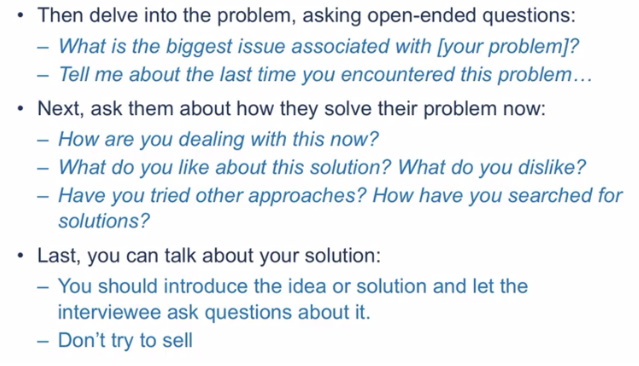
\includegraphics[width=0.8\textwidth]{./Screenshot 2025-11-17 112432.png}
              \caption{}
          \end{figure}
\end{itemize}

\subsubsection{Kesimpulan}
Mencatat hasil wawancara dan mencari pola di antara jawaban dapat memberikan umpan balik yang berguna untuk pengembangan produk. Wawancara adalah alat yang penting untuk menghindari asumsi yang salah dalam bisnis.

\subsection{Penggunaan Survei}
\begin{itemize}
    \item Survei sebaiknya dilakukan setelah wawancara untuk mendapatkan pertanyaan yang lebih baik.
    \item Survei dapat digunakan untuk meyakinkan orang lain tentang ide, tetapi lebih penting untuk menganalisis asumsi bisnis sendiri.
\end{itemize}

\subsection{Ukuran Sampel}
\begin{itemize}
    \item Semakin banyak orang yang disurvei, semakin akurat estimasi nilai yang diperoleh.
    \item Disarankan untuk survei minimal 100 orang agar hasilnya berguna.
\end{itemize}

\subsection{Metode Pengambilan Sampel}
\begin{itemize}
    \item Convenience samples: Menggunakan orang-orang yang sudah dikenal, tetapi seringkali tidak representatif.
    \item Purchase samples: Membeli data dari kelompok yang lebih acak dan representatif, seperti melalui Mechanical Turk.
    \item Iklan: Menggunakan iklan di platform seperti LinkedIn atau Facebook untuk menarik responden.
\end{itemize}

\subsection{Tips untuk Survei}
\begin{itemize}
    \item Pertanyaan demografis sebaiknya diletakkan di awal untuk membuat responden merasa nyaman.
    \item Hindari pertanyaan ya/tidak, gunakan pertanyaan dengan pilihan jawaban yang lebih beragam.
    \item Pertanyaan terbuka harus digunakan dengan hati-hati karena dapat mengurangi tingkat respons.
\end{itemize}

\subsection{Analisis Hasil Survei}
\begin{itemize}
    \item Lakukan pre-test untuk memastikan pertanyaan dipahami dengan baik.
    \item Perhatikan variasi dalam jawaban untuk mendapatkan wawasan yang lebih dalam.
    \item Bandingkan hasil survei dengan data sensus untuk memastikan representativitas sampel.
\end{itemize}

\subsection{Pengertian Prototipe (Physical Goods)}
\begin{itemize}
    \item Prototipe adalah alat untuk belajar, memecahkan masalah, dan menguji apakah solusi memenuhi kebutuhan pelanggan.
    \item Terdapat dua jenis prototipe: Prototipe Terfokus dan Prototipe Komprehensif.
\end{itemize}

\subsection{Jenis Prototipe (Physical Goods)}
\begin{itemize}
    \item Prototipe Terfokus: Mencerminkan satu atau beberapa dimensi kinerja produk, seperti mock-up atau test rigs. Contoh: prototipe alat paku tanpa fungsi yang hanya menunjukkan ukuran dan berat.
    \item Prototipe Komprehensif: Prototipe yang berfungsi penuh dan melalui beberapa tahap penyempurnaan, seperti Proof of Concept, Alpha, Beta, dan Pre-production Prototypes
\end{itemize}

\subsection{Contoh Prototipe (Physical Goods)}
\begin{itemize}
    \item Prototipe alat paku yang menunjukkan keseimbangan dan berat (Focused Prototype).
    \item Prototipe rak sepeda yang menunjukkan validitas konsep dan fungsionalitas.
\end{itemize}

\subsection{Motivasi untuk Membangun Prototipe (Physical Goods)}
\begin{itemize}
    \item Untuk tim pengembangan: belajar, memecahkan masalah, dan menguji kecocokan produk dengan pasar.
    \item Untuk audiens eksternal: membuktikan bahwa solusi berfungsi secara teknis dan bahwa pelanggan akan mengadopsi solusi tersebut.
\end{itemize}

\subsection{Strategi Kerja dengan Pemasok (Physical Goods)}
\paragraph{Model Desain Proprietary}:
\begin{itemize}
    \item Dalam model ini, Anda sebagai pengembang melakukan semua pekerjaan desain. Anda membuat gambar dan model komputer yang mendetail untuk produk yang ingin Anda buat.
    \item Pemasok kemudian memproduksi bagian tersebut sesuai dengan spesifikasi yang Anda berikan. Mereka tidak perlu tahu apa fungsi produk tersebut; mereka hanya mengikuti instruksi yang Anda berikan.
    \item Keuntungan: Anda memiliki kontrol penuh atas desain dan menjaga informasi rahasia tentang produk Anda.
    \item Kekurangan: Anda harus melakukan semua pekerjaan desain, yang bisa memakan waktu dan memerlukan keahlian khusus.
\end{itemize}
\paragraph{Model ODM (Original Design Manufacturer)}:
\begin{itemize}
    \item Dalam pendekatan ini, Anda memberikan spesifikasi fungsional kepada pemasok, dan mereka akan merancang produk untuk Anda.
    \item Pemasok memiliki keahlian dan pengalaman dalam mendesain produk yang efisien untuk diproduksi.
    \item Keuntungan: Anda tidak perlu melakukan pekerjaan desain, dan sering kali desain yang mereka buat sudah termasuk dalam biaya produksi.
    \item Kekurangan: Anda tidak memiliki hak atas desain tersebut, sehingga orang lain bisa meminta produk yang sama dari pemasok yang sama.
\end{itemize}

\subsection{Pemasok (Physical Goods)}
Pemasok adalah individu atau perusahaan yang menyediakan barang atau jasa kepada perusahaan lain. Dalam konteks pengembangan produk, pemasok biasanya merujuk pada pihak yang memproduksi komponen, bahan, atau bahkan produk jadi yang diperlukan untuk menciptakan suatu produk.

Contoh Pemasok dalam Pengembangan Produk:
\begin{itemize}
    \item Pemasok Bahan Baku: Mereka menyediakan bahan mentah yang diperlukan untuk membuat produk, seperti logam, plastik, atau bahan lainnya.
    \item Pemasok Komponen: Mereka memproduksi bagian-bagian spesifik dari produk, seperti motor, sirkuit, atau elemen mekanis lainnya.
    \item Pemasok Jasa: Mereka menawarkan layanan seperti desain, pengujian, atau produksi prototipe.
\end{itemize}

\subsection{Prototyping dalam Pengembangan Perangkat Lunak}
\begin{itemize}
    \item Prototyping membantu mengklarifikasi antarmuka pengguna dan fungsionalitas produk, mengurangi biaya dan waktu pengembangan.
    \item Melibatkan pemangku kepentingan non-teknis dalam fase prototyping dapat meningkatkan kualitas produk.
\end{itemize}

\subsection{Jenis Prototipe (Software)}
\begin{itemize}
    \item Throw Away Prototyping: Membuat model yang dapat dievaluasi oleh pengguna, kemudian dibuang setelah mendapatkan umpan balik.
    \item Evolutionary Prototyping: Mengembangkan bagian sistem yang sudah dipahami dan secara bertahap menambahkan fitur lainnya.
\end{itemize}

\subsection{Tingkat Fidelity Prototipe (Software)}
\begin{itemize}
    \item Low Fidelity: Sketsa tangan yang cepat dan memungkinkan banyak iterasi.
    \item Medium Fidelity: Keseimbangan antara kecepatan dan detail.
    \item High Fidelity: Desain mendetail yang mendekati produk akhir, memerlukan lebih banyak waktu dan sumber daya.
\end{itemize}

\subsection{Interaktivitas Prototipe (Software)}
\begin{itemize}
    \item Static Prototypes: Hanya terdiri dari serangkaian layar.
    \item Interactive Prototypes: Mampu bereaksi terhadap input pengguna, memberikan simulasi yang lebih realistis.
\end{itemize}

\subsection{Alat untuk Prototyping (Software)}
\begin{itemize}
    \item Prototipe low fidelity dapat dibuat dengan kertas dan pena.
    \item Prototipe medium hingga high fidelity dapat menggunakan alat desain seperti Photoshop atau alat wireframing seperti Balsamiq.
\end{itemize}

\subsection{Keterlibatan dalam Prototyping (Software)}
Pengusaha, bahkan tanpa keterampilan desain, sebaiknya terlibat dalam fase prototyping, terutama dalam membuat desain low fidelity.

\end{document}